\documentclass[a4paper,11pt,twoside]{memoir}
\chapterstyle{veelo}

\usepackage{TUINFDA}

\usepackage{url}
\usepackage{hyperref}					% links in pdf
\usepackage{graphicx}            			% Figures
\usepackage{verbatim}            			% Code-Environment
\usepackage[lined,linesnumbered,algochapter]{algorithm2e} % Algorithm-Environment

\usepackage{pgf}					
\usepackage{tikz}					% tikz graphics
\usetikzlibrary{arrows,automata}

\usepackage{ngerman}
\usepackage[ngerman]{babel}
\usepackage{bibgerm,cite}       % Deutsche Bezeichnungen, Automatisches Zusammenfassen von Literaturstellen
\usepackage[ngerman]{varioref}  % Querverweise
% to use the german charset include cp850 for MS-DOS, ansinew for Windows and latin1 for Linux.
% \usepackage[latin1]{inputenc}

\thesistitle{Kosteneffizientes Ressourcenmanagement in verteilten Cloud Datenzentren}{Cost aware resource management in distributed cloud data centers}
\thesissubtitle{} % optional
\thesisdate{04.03.2015}

% all titles and designations have to be gender-related!
\thesisdegree{Diplom-Ingenieur}{Master of Science}
\thesiscurriculum{Informatik}{Computer Science} % your study
\thesisverfassung{Verfasser} % Verfasser
\thesisauthor{Andreas Egger} % your name
\thesisauthoraddress{Brigittenauer Lände 224/6205, 1200 Wien} % your address
\thesismatrikelno{0626885} % your registration number

\thesisbetreins{Priv.-Doz. Dr. Ivona Brandic}
\thesisbetrzwei{Dr. Vorname Familienname}
\thesisbetrdrei{} % optional

% define page numbering styles
\makepagestyle{numberCorner}
\makeevenfoot{numberCorner}{\thepage}{}{}
\makeoddfoot{numberCorner}{}{}{\thepage}

% define custom macros for specific formats or names
\newcommand{\uml}[1]{\texttt{#1}}
\newcommand{\cd}{\textsf{Class Diagram}}

\begin{document}

\captionnamefont{\bfseries}

%%%%%%%%%%%%%%%%%%%%%%%%%%%%%%%%%%%%%%%%%
%%%   FRONTMATTER    %%%%%%%%%%%%%%%%%%%%
%%%%%%%%%%%%%%%%%%%%%%%%%%%%%%%%%%%%%%%%%
\frontmatter
\pagenumbering{roman}

%%%%%%%%%%%%%%%%%%%%%%%%%%%%%%%%%%%%%%%%%
%%%   TITLEPAGES    %%%%%%%%%%%%%%%%%%%%%
%%%%%%%%%%%%%%%%%%%%%%%%%%%%%%%%%%%%%%%%%

% the german title page is required as first page
% $Id: titlepage.tex 1752 2010-03-20 11:07:02Z tkren $
%
% TU Wien - Faculty of Informatics
% thesis titlepage
%
% This titlepage is using the geometry package, see
% <http://www.ctan.org/macros/latex/contrib/geometry/geometry.pdf>
%
% For questions and comments send an email to
% Thomas Krennwallner <tkren@kr.tuwien.ac.at>
% or to Petra Brosch <brosch@big.tuwien.ac.at>
%

\selectlanguage{ngerman}

% setup page dimensions for titlepage
\newgeometry{left=2.4cm,right=2.4cm,bottom=2.5cm,top=2cm}

% force baselineskip and parindent
\newlength{\tmpbaselineskip}
\setlength{\tmpbaselineskip}{\baselineskip}
\setlength{\baselineskip}{13.6pt}
\newlength{\tmpparindent}
\setlength{\tmpparindent}{\parindent}
\setlength{\parindent}{17pt}

% first titlepage
\thispagestyle{tuinftitlepage}

%
% Kludge: for each titlepage set \pagenumbering to a different
% style. This is used to fix a problem with hyperref, because there
% are multiple "page 1" and hyperref hates that
%
\pagenumbering{Alph}

\begin{center}
{\ \vspace{3.4cm}}

\begin{minipage}[t][2.8cm][s]{\textwidth}%
\centering
\thesistitlefontHUGE\sffamily\bfseries\tuinfthesistitle\\
\bigskip
{\thesistitlefonthuge\sffamily\bfseries\tuinfthesissubtitle}
\end{minipage}

\vspace{1.3cm}

{\thesistitlefontLARGE\sffamily \tuinfthesistype}

\vspace{6mm}

{\thesistitlefontlarge\sffamily zur Erlangung des akademischen Grades}

\vspace{6mm}

{\thesistitlefontLARGE\sffamily\bfseries \tuinfthesisdegree}

\vspace{6mm}

{\thesistitlefontlarge\sffamily im Rahmen des Studiums}

\vspace{6mm}

{\thesistitlefontLarge\sffamily\bfseries \tuinfthesiscurriculum}

\vspace{6.5mm}

{\thesistitlefontlarge\sffamily eingereicht von}

\vspace{6mm}

{\thesistitlefontLarge\sffamily\bfseries \tuinfthesisauthor}

\vspace{1.5mm}

{\thesistitlefontlarge\sffamily Matrikelnummer \tuinfthesismatrikelno} 

\vspace{1.4cm}

\vspace{0pt}\raggedright\thesistitlefontnormalsize\sffamily
\begin{minipage}[t][1.6cm][t]{\textwidth}%
  %
  an der

  Fakult\"{a}t f\"{u}r Informatik der Technischen Universit\"{a}t Wien
\end{minipage}

\begin{minipage}[t][4cm][t]{\textwidth}%
  \vspace{0pt}\raggedright\thesistitlefontnormalsize\sffamily
  %
  \begin{tabbing}%
	    \hspace{19mm} \= \hspace{66mm} \kill
	    \tuinfthesisbetreuung: \> \tuinfthesisbetreins\\
	    Mitwirkung: \> \tuinfthesisbetrzwei\\
	                \> \tuinfthesisbetrdrei
  \end{tabbing}
\end{minipage}

\begin{minipage}[t][1.5cm][t]{\textwidth}%
  \vspace{0pt}\sffamily\thesistitlefontnormalsize
  \begin{tabbing}%
    \hspace{45mm} \= \hspace{63mm} \= \hspace{51mm} \kill
    Wien, \tuinfthesisdate \> {\raggedright\rule{51mm}{0.5pt}} \> {\raggedright\rule{51mm}{0.5pt}} \\
    \> \begin{minipage}[t][0.5cm][t]{51mm}\centering (Unterschrift \tuinfthesisverfassung)\end{minipage}
    \> \begin{minipage}[t][0.5cm][t]{51mm}\centering (Unterschrift \tuinfthesisbetreuung)\end{minipage}
    \end{tabbing}
\end{minipage}

\end{center}

% we want an empty page right after first titlepage
\pagestyle{empty}
\cleardoublepage

% we're done with the titlepages, proceed with default pagenumbering
\pagenumbering{roman}

% restore baselineskip
\setlength{\baselineskip}{\tmpbaselineskip}
\setlength{\parindent}{\tmpparindent}

% back to normal geometry
\restoregeometry

\selectlanguage{english}

%%% Local Variables:
%%% TeX-PDF-mode: t
%%% TeX-debug-bad-boxes: t
%%% TeX-parse-self: t
%%% TeX-auto-save: t
%%% reftex-plug-into-AUCTeX: t
%%% End:


% an english translation may follow
% $Id: titlepage.tex 1752 2010-03-20 11:07:02Z tkren $
%
% TU Wien - Faculty of Informatics
% thesis titlepage
%
% This titlepage is using the geometry package, see
% <http://www.ctan.org/macros/latex/contrib/geometry/geometry.pdf>
%
% For questions and comments send an email to
% Thomas Krennwallner <tkren@kr.tuwien.ac.at>
% or to Petra Brosch <brosch@big.tuwien.ac.at>
%

% setup page dimensions for titlepage
\newgeometry{left=2.4cm,right=2.4cm,bottom=2.5cm,top=2cm}

% force baselineskip and parindent
%\newlength{\tmpbaselineskip}
%\setlength{\tmpbaselineskip}{\baselineskip}
%\setlength{\baselineskip}{13.6pt}
%\newlength{\tmpparindent}
%\setlength{\tmpparindent}{\parindent}
%\setlength{\parindent}{17pt}

% first titlepage
\thispagestyle{tuinftitlepage}

%
% Kludge: for each titlepage set \pagenumbering to a different
% style. This is used to fix a problem with hyperref, because there
% are multiple "page 1" and hyperref hates that
%
\pagenumbering{Roman}

\begin{center}
{\ \vspace{3.4cm}}

\begin{minipage}[t][2.8cm][s]{\textwidth}%
\centering
\thesistitlefontHUGE\sffamily\bfseries\tuinfthesistitle\\
\bigskip
{\thesistitlefonthuge\sffamily\bfseries\tuinfthesissubtitle}
\end{minipage}

\vspace{1.3cm}

{\thesistitlefontLARGE\sffamily \tuinfthesistypeen}

\vspace{6mm}

{\thesistitlefontlarge\sffamily submitted in partial fulfillment of the requirements for the degree of}

\vspace{6mm}

{\thesistitlefontLARGE\sffamily\bfseries \tuinfthesisdegreeen}

\vspace{6mm}

{\thesistitlefontlarge\sffamily in}

\vspace{6mm}

{\thesistitlefontLarge\sffamily\bfseries \tuinfthesiscurriculumen}

\vspace{6.5mm}

{\thesistitlefontlarge\sffamily by}

\vspace{6mm}

{\thesistitlefontLarge\sffamily\bfseries \tuinfthesisauthor}

\vspace{1.5mm}

{\thesistitlefontlarge\sffamily Registration Number \tuinfthesismatrikelno} 

\vspace{1.4cm}

\begin{minipage}[t][1.6cm][t]{\textwidth}%
  \vspace{0pt}\raggedright\thesistitlefontnormalsize\sffamily
  %
  to the Faculty of Informatics 

  at the Vienna University of Technology
\end{minipage}

\vspace{0pt}\raggedright\thesistitlefontnormalsize\sffamily
\begin{minipage}[t][4cm][t]{\textwidth}%
  \begin{tabbing}%
	    \hspace{19mm} \= \hspace{66mm} \kill
	    Advisor: \> \tuinfthesisbetreins\\
	    Assistance: \> \tuinfthesisbetrzwei\\
	                \> \tuinfthesisbetrdrei
     \end{tabbing}
\end{minipage}

\begin{minipage}[t][1.5cm][t]{\textwidth}%
  \vspace{0pt}\sffamily\thesistitlefontnormalsize
  \begin{tabbing}%
    \hspace{45mm} \= \hspace{63mm} \= \hspace{51mm} \kill
    Vienna, \tuinfthesisdate \> {\raggedright\rule{51mm}{0.5pt}} \> {\raggedright\rule{51mm}{0.5pt}} \\
    \> \begin{minipage}[t][0.5cm][t]{51mm}\centering (Signature of Author)\end{minipage}
    \> \begin{minipage}[t][0.5cm][t]{51mm}\centering (Signature of Advisor)\end{minipage}
    \end{tabbing}
\end{minipage}

\end{center}

% we want an empty page right after first titlepage
\pagestyle{empty}
\cleardoublepage

% we're done with the titlepages, proceed with default pagenumbering
\pagenumbering{roman}

% restore baselineskip
\setlength{\baselineskip}{\tmpbaselineskip}
\setlength{\parindent}{\tmpparindent}

% back to normal geometry
\restoregeometry


%%% Local Variables:
%%% TeX-PDF-mode: t
%%% TeX-debug-bad-boxes: t
%%% TeX-parse-self: t
%%% TeX-auto-save: t
%%% reftex-plug-into-AUCTeX: t
%%% End:
 % optional

%%%%%%%%%%%%%%%%%%%%%%%%%%%%%%%%%%%%%%%%%
%%%   ERKLAERUNG DER SELBSTAENDIGKEIT   %
%%%%%%%%%%%%%%%%%%%%%%%%%%%%%%%%%%%%%%%%%
\cleardoublepage
\selectlanguage{ngerman}
\chapter*{Erklärung zur Verfassung der Arbeit}

\tuinfthesisauthor\\
\tuinfthesisauthoraddress

\vspace*{1.2cm}

Hiermit erkläre ich, dass ich diese Arbeit selbständig verfasst habe, 
dass ich die verwendeten Quellen und Hilfsmittel vollständig angegeben 
habe und dass ich die Stellen der Arbeit - einschließlich Tabellen, 
Karten und Abbildungen -, die anderen Werken oder dem Internet im 
Wortlaut oder dem Sinn nach entnommen sind, auf jeden Fall unter Angabe 
der Quelle als Entlehnung kenntlich gemacht habe.\\

\vspace*{2cm}
\begin{tabbing}%
    \hspace{58mm} \= \hspace{28mm} \= \hspace{58mm} \kill
    {\raggedright\rule{58mm}{0.5pt}} \> \> {\raggedright\rule{58mm}{0.5pt}} \\
    \begin{minipage}[t][0.5cm][t]{58mm}
	\vspace{0pt}\sffamily\thesistitlefontnormalsize
	\centering (Ort, Datum)
    \end{minipage}
    \> \>
    \begin{minipage}[t][0.5cm][t]{58mm}
	\vspace{0pt}\sffamily\thesistitlefontnormalsize
	\centering (Unterschrift \tuinfthesisverfassung)
    \end{minipage}
\end{tabbing}


\selectlanguage{english}

%%%%%%%%%%%%%%%%%%%%%%%%%%%%%%%%%%%%%%%%%
%%%   ACKNOWLEDGEMENTS    %%%%%%%%%%%%%%%
%%%%%%%%%%%%%%%%%%%%%%%%%%%%%%%%%%%%%%%%%

% optional acknowledgements may be included in german or in english
%\chapter*{Danksagung}

Hier fügen Sie optional eine Danksagung ein.
 		% optional
\chapter*{Acknowledgements}

Optional acknowledgements may be inserted here.	% optional

%%%%%%%%%%%%%%%%%%%%%%%%%%%%%%%%%%%%%%%%%
%%%   ABSTARCT    %%%%%%%%%%%%%%%%%%%%%%%
%%%%%%%%%%%%%%%%%%%%%%%%%%%%%%%%%%%%%%%%%

\chapter*{Abstract}

Cloud computing services experienced increasing popularity over the recent years which caused the power demand of data centers to increase significantly. 
As energy costs represent a significant part of the total cost of data centers energy cost reductions in cloud computing environments play an important role for cloud providers to remain competitive and provide affordable cloud services. This thesis introduces a cloud framework to evaluate energy cost reductions in multi electricity market environments. It is shown that substantial cost savings are possible using intelligent resource scheduling algorithms with integration of energy price forecasts. 

This thesis consists of two parts. In the first part different forecasting models are evaluated to assess the performance of the models for energy price time series of different energy markets. A forecast simulation framework is introduced capable of dynamically managing energy price data from different power markets and generating forecasts based on that data. The framework incorporates methods for automatic model generation and evaluation as a basis for extended forecast simulations. 
A large scale forecast evaluation is conducted to gain insights into model accuracy across a wide range of energy price data. Different training periods, forecast horizons and energy price datasets lead to a comprehensive evaluation of the forecasting models. 

The second part is dedicated to large scale cloud simulations comprising different cloud schedulers and scenarios. An existing cloud simulation framework has been extended to perform simulations across a wide range of energy price data where different scheduling mechanisms have been introduced. 
A utility function has been defined for sophisticated evaluation of different criteria to decide on the best suitable VMs to migrate at any point in time. Criteria involve probability of SLA penalties and maximum cost benefits to appropriately handle the tradeoff between minimizing costs and providing an adequate level of quality of service. 

Results show that significant cost savings are possible with schedulers incorporating different criteria and energy price forecasts revealing promising results. Based on the defined cloud settings it illustrates the applicability of the proposed approach to real world scenarios of geo-distributed data centers connected to energy markets. 



\cleardoublepage
\selectlanguage{ngerman}
\chapter*{Kurzfassung}

Hier fügen Sie die Kurzfassung auf Deutsch gemäß den Vorgaben der Fakultät ein.

\selectlanguage{english}

%%%%%%%%%%%%%%%%%%%%%%%%%%%%%%%%%%%%%%%%%
%%%   CONTENTS    %%%%%%%%%%%%%%%%%%%%%%%
%%%%%%%%%%%%%%%%%%%%%%%%%%%%%%%%%%%%%%%%%
% uncomment to set document language to german (results in "Inhaltsverzeichnis", "Kapitel", "Abbildung", etc. instead of "Contents", "Chapter", and "Figure"), otherwise the document's language is english
%\selectlanguage{ngerman}

\setcounter{tocdepth}{1}

\cleardoublepage
\pagestyle{numberCorner}
\tableofcontents*

%%%%%%%%%%%%%%%%%%%%%%%%%%%%%%%%%%%%%%%%%
%%%   MAINMATTER    %%%%%%%%%%%%%%%%%%%%%
%%%%%%%%%%%%%%%%%%%%%%%%%%%%%%%%%%%%%%%%%

\mainmatter
\pagenumbering{arabic}
\pagestyle{numberCorner}


%%%%%%%%%%%%%%%%%%%%%%%%%%%%%%%%%%%%%%%%%
\chapter{Thesis Template}
\label{ch:template}
%%%%%%%%%%%%%%%%%%%%%%%%%%%%%%%%%%%%%%%%%

\section{General Information}

This document is intended as a template and guideline and should support the author in the course of doing the master's thesis.
Assessment criteria comprise the quality of the theoretical and/or practical work as well as structure, content and wording of the written master's thesis. Careful attention should be given to the basics of scientific work (e.g., correct citation).

\section{Organizational Issues}

A master's thesis at the Faculty of Informatics has to be finished within six months. During this period regular meetings between the advisor(s) and the author have to take place.
In addition, the following milestones have to be fulfilled:
\begin{enumerate}
  \item  Within one month after having fixed the topic of the thesis the master's thesis proposal has to be prepared and must be accepted by the advisor(s). The master's thesis proposal must follow the respective template of the dean of academic affairs. Thereafter the proposal has to be applied for at the deanery. The necessary forms may be found on the web site of the Faculty of Informatics. \url{http://www.informatik.tuwien.ac.at/dekanat/formulare.html}
  \item  Accompanied with the master's thesis proposal, the structure of the thesis in terms of a table of contents has to be provided.
  \item Then, the first talk has to be given at the so-called ``Seminar for Master Students''. The slides have to be discussed with the advisor(s) one week in advance. Attendance of the ``Seminar for Master Students'' is compulsory and offers the opportunity to discuss arising problems among other master students.
  \item At the latest five months after the beginning, a provisional final version of the thesis has to be handed over to the advisor(s).  
  \item As soon as the provisional final version exists, a first poster draft has to be made. The making of a poster is a compulsory part of the ``Seminar for Master Students'' for all master studies at the Faculty of Informatics. Drafts and design guidelines can be found at \url{http://www.informatik.tuwien.ac.at/studium/richtlinien}.
  \item After having consulted the advisor(s) the second talk has to be held at the ``Seminar for Master Students''.
  \item At the latest six months after the beginning, the corrected version of the master's thesis and the poster have to be handed over to the advisor(s).
  \item After completion the master's thesis has to be presented at the ``epilog''. For detailed information on the epilog see: \\ \url{http://www.informatik.tuwien.ac.at/studium/epilog}
\end{enumerate}

\section{Structure of the Master's Thesis}

If the curriculum regulates the language of the master's thesis to be English (like for ``Business Informatics''), the thesis has to be written in English. Otherwise, the master's thesis may be written in English or in German. The structure of the thesis is predetermined.
The table of contents is followed by the introduction and the main part, which can vary according to the content. The master's thesis ends with the bibliography (compulsory) and the appendix (optional).

\begin{itemize}
  \item	Cover page
  \item Acknowledgements
  \item Abstract of the thesis in English and German
  \item Table of contents
  \item Introduction
  	\begin{itemize}
  		\item motivation
  		\item problem statement (which problem should be solved?)
  		\item aim of the work
  		\item methodological approach
  		\item structure of the work
  	\end{itemize}
  \item State of the art / analysis of existing approaches
  	\begin{itemize}
  		\item literature studies
  		\item analysis
  		\item comparison and summary of existing approaches
  	\end{itemize}
  \item Methodology
  	\begin{itemize}
  		\item used concepts
  		\item methods and/or models
  		\item languages
  		\item design methods
  		\item data models
  		\item analysis methods
  		\item formalisms
  	\end{itemize}
  \item Suggested solution/implementation
  \item Critical reflection
  	\begin{itemize}
  		\item comparison with related work
  		\item discussion of open issues
  	\end{itemize}
  \item Summary and future work
  \item Appendix: source code, data models, \dots
  \item Bibliography
\end{itemize}



%%%%%%%%%%%%%%%%%%%%%%%%%%%%%%%%%%%%%%%%%
\chapter{Introduction}
\label{ch:intro}
%%%%%%%%%%%%%%%%%%%%%%%%%%%%%%%%%%%%%%%%%



\section{Motivation}

In times of cloud computing where computer resources are expected to be readily available from anywhere \cite{buyya2009cloud} and with an ever growing global network of interconnected devices cloud providers need to cope with increasing energy consumption in data centers as requests need to be handled at a rapid pace. 
As energy consumption is directly mapped to energy costs, cloud providers aim to reduce power consumption and thus electricity costs within data centers. 

Studies show that electricity costs for cloud systems comprising several large scale data centers is in the range of tens of millions of dollars per year \cite{qureshi2009cutting}. Energy consumption, related energy costs and high energy prices may slow down or hinder advancements in cloud computing. Thus, cloud providers must ensure that delivering their services remains profitable. Lower energy costs increase the competitive ability of cloud providers and bigger investments are possible. Likewise customers may benefit from more affordable cloud services. 

Energy cost reductions can be addressed by utilizing one of two different approaches. One common approach is to increase energy efficiency in data centers to reduce energy consumption and therefore energy related costs as well [c]. This is done i.e.~by utilizing more energy efficient hardware, implementing an energy efficient cooling system, virtualization of servers or energy aware load distribution policies. It additionally aims at minimizing the Power Usage Effectiveness (PUE) of data centers which describes the ratio of the total amount of power consumed to the power consumed solely by IT equipment\footnote{http://www.itwissen.info/definition/lexikon/power-usage-effectivness-PUE.html} [r]. Despite the importance of increasing energy efficiency to reduce costs and environmental load this approach is limited as energy efficiency may not be improved beyond a critical point where investments in energy efficiency measures do not further reduce overall energy expenses [g]. 
%Thus the expenses of auxiliary systems should be reduced to a minimum to spend less on electricity. 
%Two common approaches address the reduction of energy costs in data centers. 

The second approach is directed at intelligent scheduling mechanisms based on dynamically changing energy prices. In wholesale power markets energy prices commonly change at an hourly basis with factors up to 10 from one hour to the next [c]. Electricity price behavior of power markets may differ significantly with possibly involved seasonality patterns where different time zones lead to substantial locational price differences. These characteristics of locational and temporal varying energy prices may be exploited by intelligent scheduling algorithms and cost aware resource management routines that place requests at facilities currently exhibiting low energy prices. In addition the current energy price time series at any location and time stamp is observed and resources may be migrated to data centers that currently operate below peak load and facing low energy prices. %where energy prices are currently cheaper. 

The focus of this thesis is to go beyond intelligent scheduling of resources %to fit the current distribution of energy prices 
by integrating sophisticated forecasting methods that predict price time series behaviors into the near future. This measure is expected to further optimize resource distribution across data centers by comparing and analyzing current and predicted energy price time series to find the best fit of resources in the near future which should result in the maximum possible energy cost reduction.

%The goal of this thesis is to reduce energy related costs of interconnected data centers with respect to changing energy prices in wholesale power markets. 
%The proposed approach is to optimize load placement and migration between data centers considering time and location based energy prices. 
%In addition to placing resources at locations currently facing low energy prices the resources or virtual machines are migrated to sites where low energy prices are \emph{expected} in the near future. 

%The scenario includes data centers located in different countries where different energy markets and prices apply. Thus constellations may arise where it is profitable to migrate a certain amount of resources from a data center facing high energy prices to a data center where energy prices are low at the current point in time or in the near future. 

\section{Problem Statement}

Energy prices are traded and change hourly within the energy markets, so investigations need to be made in order to make qualified statements about the estimated energy price at some point in time in the near future.
This is done by analyzing historical price data and building models for accurate energy price forecasting. Energy prices belonging to different energy markets are estimated for various time ranges into the future. Based upon the results it is decided how many resources may be migrated currently or in the future in order to obtain the maximum possible energy cost reduction. 
However, forecasting errors represented by the difference between estimated and real energy prices increase with the length of the estimation window which has to be taken into account when determining the length of the forecasting window. 

Since energy prices change dynamically a flexible approach of moving data center resources to more cost-effective locations is needed. This work is based on the scenario of a company running data centers distributed across several countries. Depending on the current and estimated energy price for a certain region resources may be relocated to other data centers located at more cost-effective regions.

The key technology to implement the relocation of data center resources is virtual machine (VM) migration \cite{nelson2009virtual}. All data and services are located on servers and belong to specific virtual machines within a data center. Since a server may host several VMs that operate completely independent from each other, they can be relocated (migrated) to other servers, possibly over networks without affecting VMs running on the same server. VM migration may be applied across large geographical distances (geo migrations) by leveraging connections via the internet. It is also possible to do live migrations on a large scale without noticeable service interruption \cite{celesti2010improving}. 

Various load policies exist to optimize the load factor and distribution of tasks within data centers \cite{buyya2010energy}. A workload manager has to make sure that there are still servers having enough resources and no service level agreement (SLA) is violated on the assignment of a new job. 
In contrast, this work aims to optimize workload distribution among geographically distributed data centers with a focus on the reduction of overall electricity costs. This is done by intelligent scheduling while utilizing forecasting methods and predicting energy prices within the near future. 
Furthermore, by considering the history of energy prices and resource load within a certain region it is estimated whether or not a migration to another data center makes sense regarding the current load and configuration. Therefore, forecasting methods in combination with machine learning techniques will be evaluated and applied to the scenario. 

\section{Aim of the work}

The goal of this thesis is to show ways for data center operators in charge of geographically distributed and interconnected data centers to save on their power bill by exploiting VM migrations and the variability of energy prices in wholesale power markets. This approach presumes that data center operators are charged directly by wholesale power markets, which can be a suitable option since power market integration can effectively increase the power usage efficiency (PUE) within a data center\footnote{Data Center Trends: Optimizing power markets \url{http://www.datacenterworld.com/fall2013/account/Uploader/uploader\_files/show/335/}}. Given the fact that data centers consume a huge amount of energy comparable to the energy consumption of small cities\cite{qureshi2009cutting} it becomes a viable option for them to be integrated into wholesale energy markets. By leveraging the technique of resource migration to data centers where cheaper energy prices apply at the current point in time significant savings in energy bills are possible while still maintaining a defined level of quality of service. 

Initially placing resources at data centers that currently exhibit cheap energy prices can reduce energy expenses significantly compared to a non power aware approach. Combined with energy price forecasts resources may be scheduled intelligently such that price changes within the near future can be detected and resources are placed with respect to the estimated prices. This approach may be evaluated against an ad-hoc approach where resources are assigned to data centers by only considering current energy prices and workload. 

A simulation scenario will be established where workload is placed on several geographically distributed and interconnected data centers and results are evaluated based on the given workload, energy prices and data center capacities. In addition, energy price forecasts will be integrated to predict significant changes in energy price levels at different energy markets. This should lead to a more cost efficient scheduling approach where workload is placed at data centers which provide best energy price conditions for current and/or future time spots. 

The simulation will be based on a well established cloud scheduler\footnote{\url{http://philharmonic.github.io/}} with set parameters to simulate a predefined scenario. The results for different scenarios and parameter settings (i.e.~with or without forecasts) will be compared and evaluated such that the possible benefits and drawbacks of each of these approaches can be examined. 
In addition to energy prices and workload this scheduler may take into account cooling costs related to ambient temperatures which can take up a significant part of data center expenses. 

A special focus will be laid on evaluating energy price forecasting methods to find the best fit for the given data and scenarios. For the simulation there will be a focus on short term price forecasting, as energy price levels change rapidly within energy markets and exhibit a very volatile nature. Therefore accurate price forecasting is only possible when applied to short term forecasts. 
Different forecasting methods will be compared by accuracy and error measures to determine the most suitable forecasting horizon and parameter settings for various models and data. It is expected that through good quality forecasting the results of the simulation in terms of energy costs can be improved significantly. This should help cloud providers to save on their energy bills and provide more efficient scheduling of cloud related data. 

\section{Methodological Approach}

The proposed scenario consists of a private cloud with data centers located in countries where participation in power markets is possible and energy price data is available. The geographical location and connections between data centers should be defined such that VM migrations may be done interchangeably. 

To maximize the predictive accuracy of price forecasting different parameters of forecasting methods should be evaluated and compared to determine the settings with the most accurate results in each case. The accuracy should be evaluated for various time ranges on both in-sample and out-of-sample forecasts and each location and time series separately. Due to the volatile nature of hourly real time energy prices there is a natural boundary of about 48 hours up to which forecasts can be made with reasonable accuracy. Models should be trained and compared based on forecast error measures on in-sample data (i.e.~MAPE) to determine the most accurate models. 

As a next step a model is to be defined for the simulation with parameters needed for further operation. For example, the amount of bandwidth between two data centers needs to be set and a method for calculating the cost of VM migration has to be defined, depending on current energy prices. Furthermore the minimum number of VMs should be set that may be migrated in order to compensate for migration costs. 

Regarding forecasting models there is evidence that some models are generally more suitable for energy price forecasting than others \cite{weron2008forecasting}\cite{weron2005forecasting}. For example, for averaged short term forecasts a common model to use is simple exponential smoothing (SES) which averages out any variations in the data and provides a good stationary estimate of future data values. In many cases this generates results with sufficient accuracy due to a strong irregular component (random fluctuations) in the data set. 

Another common model for price forecasting is the ARIMA model which may contain both an auto-regressive (AR) and moving-average (MA) part and can thus be applied to various data sets depending on the chosen parameters. Also, various forms of auto-regressive models exist which may provide a good fit for mid term forecasting. 
Therefore representatives from each of these models will be chosen where the focus lies on predicting real-time energy prices as they are collected on an hourly basis in contrast to the day-ahead spot energy prices which are provided for the next 24 hours simultaneously. 

\section{Structure of the work}

The structure of this thesis consists of five main parts. 

In the introduction a general outline is described comprising the purpose of the thesis, the problem statement and how these problems are solved within the thesis. Short insights are given into proposed methodologies and how they are expected to provide improvements to the outlined scenario. 

State of the art discusses relevant literature in the field with a comprehensive collection of related articles and journals. It is examined what kind of advancement in the different fields have been made in the past that relate to this thesis and how they can be used as a basis for further investigations. After a detailed analysis of the different approaches of solving problems in the respective field the approaches are compared and summarized to discuss what is still missing and can be improved upon or further investigated. 

Methodology comprises definitions and concepts used in further chapters and provides the basis for the discussion of the proposed solution. It investigates in detail theoretical models and concepts which were derived from extensive research in the field. It gives an overview of different energy markets, their inherent characteristics and related energy price time series behavior. The characteristics of electricity prices in wholesale power markets is discussed, as well as different pricing models applicable to these markets. State of the art data centers are investigated to get an idea of the possibilities and limitations of these systems. Finally relevant forecasting models and their theoretical background are discussed to better understand their applications within the thesis. 

The suggested solution or implementation shows the results and outcome of the research in previous chapters. It comprises the general idea and background for the proposed approach, a description of the technical architecture and structure of the implementation and possible interaction with other systems or components. The model selection process is explained in detail and how it contributes to the overall solution. This is crucial as good quality forecasting depends on the goodness of fit of the model in relation to the given data or time series. The empirical evaluation chapter describes the application of selected models to the framework and its behavior when assigned to real world data from different power markets. 
An important part of the evaluation is done on a simulator that mimics a cloud environment consisting of several distributed data centers. Considering changing energy prices, ambient temperatures, cooling efficiencies, scheduling of virtual machines combined with energy price forecasting it can provide comprehensive insights on possible cost reductions by applying forecasting in cloud environments. 

The discussion and critical reflection contains an overall discussion and investigation of the proposed solution and its possible benefits and limitations. It is compared to related work and how it fits into current research topics. Potential improvements to the proposed implementation are discussed with a reference of open issues. 
Finally the results are summarized and potential future advancements in achieving cost reductions in cloud environments are estimated. A future outlook concludes the work. 




%%%%%%%%%%%%%%%%%%%%%%%%%%%%%%%%%%%%%%%%%
\chapter{State of the Art}
\label{ch:related_work}
%%%%%%%%%%%%%%%%%%%%%%%%%%%%%%%%%%%%%%%%%

\section{Electricity markets and pricing}

In wholesale energy markets different pricing and bidding models can be used. 

Currently the two most common price evaluation strategies are day-ahead and real-time pricing strategies. 

In \cite{uniform2008tierney} two different bidding strategies are discussed, uniform pricing and pay-as-bid auctions. In the uniform pricing model the market clearing price is determined by collecting the marginal prices from all suppliers and taking the maximum price from this collection. Conversely, in pay-as-bid auctions a supplier gets paid based on its actual bid. 



%%%%%%%%%%%%%%%%%%%%%%%%%%%%%%%%%%%%%%%%%
\chapter{Typographic Design}
\label{ch:typo}
%%%%%%%%%%%%%%%%%%%%%%%%%%%%%%%%%%%%%%%%%


For working with LaTeX you can take advantage of a variety of books and free introductions and tutorials on the internet. A competent contact point for LaTeX beginners is the LaTeX Wikibook, which is available under \url{http://en.wikibooks.org/wiki/LaTeX}. 

The following sections give examples of the most important LaTeX environments and commands.

\section{Tables}

Tables have to be realized with the help of the \textit{table} environment. Tables shall be sequentially numbered for each chapter and described in terms of a short caption (cf. Table~\ref{tab:diplomaseminar}).

\begin{table}[htb]
	\centering
	\begin{tabular}{|l|c|c|}
		\hline \textbf{Name} & \textbf{Date} & \textbf{Title} \\
		\hline
		\hline Mustermann Adam  & 18.5   & T1    \\
		\hline Musterfrau Eva  & 22.6   & T2    \\
		\hline
	\end{tabular}
	\caption{Seminar for Master Students}
	\label{tab:diplomaseminar}
\end{table}


\section{Figures}

Like tables, figures shall be sequentially numbered for each chapter and described in terms of a short caption). You could either produce your drawings directly inside Latex using PSTricks\footnote{\url{http://tug.org/PSTricks}}, Tikz\footnote{\url{http://sourceforge.net/projects/pgf}}, or any set of macros dedicated to your requirements (cf. Figure~\ref{fig:samplefigure_tikz}). Alternatively, you may include figures prepared in external tools (cf. Figure~\ref{fig:samplefigure_pdf}). Note, to ensure high quality printing, all figures must have at least 300 dpi.

\begin{figure}
	\centering
	\begin{tikzpicture}[->, auto, node distance=2.8cm, semithick]
	  \node[initial, state] (1)		 {$S_1$};
	  \node[state] 		(2) [right of=1] {$S_2$};
	
	  \path (1) edge [bend left]  node {0} (2)
		(1) edge [loop above] node {1} (1)
		(2) edge [bend left]  node {0} (1)
		(2) edge [loop above] node {1} (2);
	\end{tikzpicture}
	\caption{Sample figure}
	\label{fig:samplefigure_tikz}
\end{figure}

\begin{figure}[tb]
	\centering
	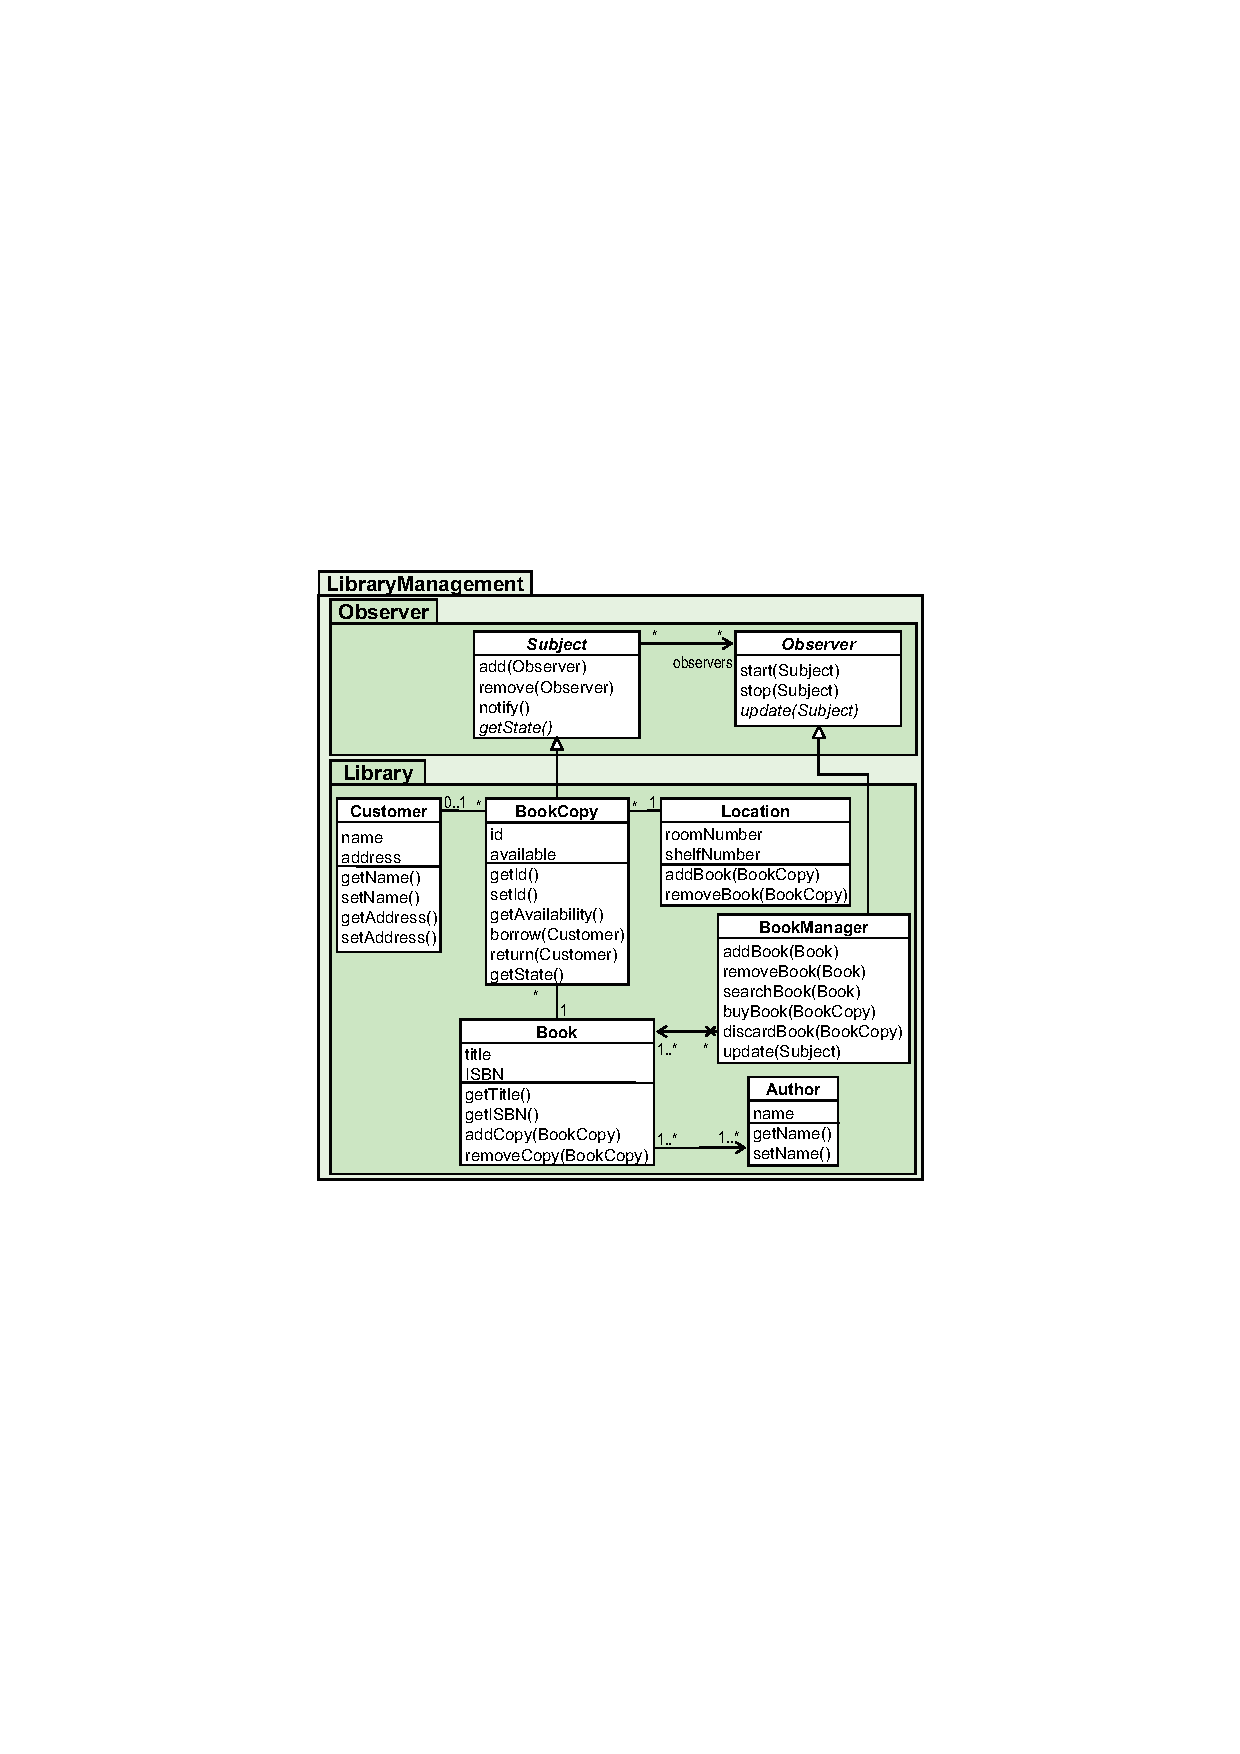
\includegraphics[width=0.7\textwidth]{figures/figure1}
	\caption{Sample figure}
	\label{fig:samplefigure_pdf}
\end{figure}


\section{Fonts}

When introducing important terms for the first time use \emph{emphasize}. For a consistent look and feel of proper names like {\cd} and {\uml{Observer}} pattern you may define macros in the main document \texttt{thesis.tex}.

\section{Code}

For short code fragments use the \textit{verbatim} environment.

\begin{verbatim}
//Start Program
System.out.println("Hello World!");
//End Program
\end{verbatim}

A much better alternative is the \textit{algorithm} environment (cf. Algorithm~\ref{alg:samplealgorithm}). This environment offers special formatting features for loops, operations and comments.

\begin{algorithm}[t]
\SetKwData{Left}{left}
\SetKwData{This}{this}
\SetKwData{Up}{up}
\SetKwFunction{Union}{Union}
\SetKwFunction{FindCompress}{FindCompress}
\SetKwInOut{Input}{input}
\SetKwInOut{Output}{output}

\Input{A bitmap $Im$ of size $w\times l$}
\Output{A partition of the bitmap}

\BlankLine

\emph{special treatment of the first line}\;
\For{$i\leftarrow 2$ \KwTo $l$}{
\emph{special treatment of the first element of line $i$}\;
\For{$j\leftarrow 2$ \KwTo $w$}{\label{forins}
\Left$\leftarrow$ \FindCompress{$Im[i,j-1]$}\;
\Up$\leftarrow$ \FindCompress{$Im[i-1,]$}\;
\This$\leftarrow$ \FindCompress{$Im[i,j]$}\;
\If(\tcp*[r]{O(\Left,\This)==1}){\Left compatible with \This}{\label{lt}
\lIf{\Left $<$ \This}{\Union{\Left,\This}}\;
\lElse{\Union{\This,\Left}\;}
}
\If(\tcp*[r]{O(\Up,\This)==1}){\Up compatible with \This}{\label{ut}
\lIf{\Up $<$ \This}{\Union{\Up,\This}}\;
\tcp{\This is put under \Up to keep tree as flat as possible}\label{cmt}
\lElse{\Union{\This,\Up}}\tcp*[r]{\This linked to \Up}\label{lelse}
}
}
\lForEach{element $e$ of the line $i$}{\FindCompress{p}}
}
\caption{Sample algorithm}\label{alg:samplealgorithm}
\end{algorithm}



%%%%%%%%%%%%%%%%%%%%%%%%%%%%%%%%%%%%%%%%%
\chapter{Bibliographic Issues}
\label{ch:bibliographic}
%%%%%%%%%%%%%%%%%%%%%%%%%%%%%%%%%%%%%%%%%

\section{Literature Search}

Information on online libraries and literature search, e.g., interesting magazines, journals, conferences, and organizations may be found at \url{http://www.big.tuwien.ac.at/teaching/info.html}.

\section{BibTeX}

BibTeX should be used for referencing.

The LaTeX source document of this pdf document provides you with different samples for references to journals~\cite{jour:B2BServices}, conference papers~\cite{proc:TheWebMLApproach}, books~\cite{book:umlatwork}, book chapters~\cite{incoll:ErhardKonrad1992}, electronic standards~\cite{man:BPEL}, dissertations~\cite{phdthesis:manuelWimmer}, masters' theses~\cite{mast:AUMLProfile}, and web sites~\cite{misc:BIGWebsite}. The respective BibTeX entries may be found in the file \texttt{references.bib}. For administration of the BibTeX references we recommend \url{http://www.citeulike.org} or JabRef for offline administration, respectively.


%%%%%%%%%%%%%%%%%%%%%%%%%%%%%%%%%%%%%%%%%
%%% BACKMATTER %%%%%%%%%%%%%%%%%%%%%%%%%%
%%%%%%%%%%%%%%%%%%%%%%%%%%%%%%%%%%%%%%%%%

\appendix

\bibliographystyle{plain}
\bibliography{references}

\end{document}
